\section{Implementation}

The proposed service consists of several aspects: A interface for tablet computers; streaming of video; programme recommendations; advert campaigns \& uploading; advert selection and the general architecture of the service.

In the following section, the technical details of the implemented system, \textit{Your4.tv}, will be discussed. This includes the overall systems architecture, database design, and the languages and tools used during the development process.

\subsection{Systems architecture and description}

\begin{figure}[H]
	\centering
	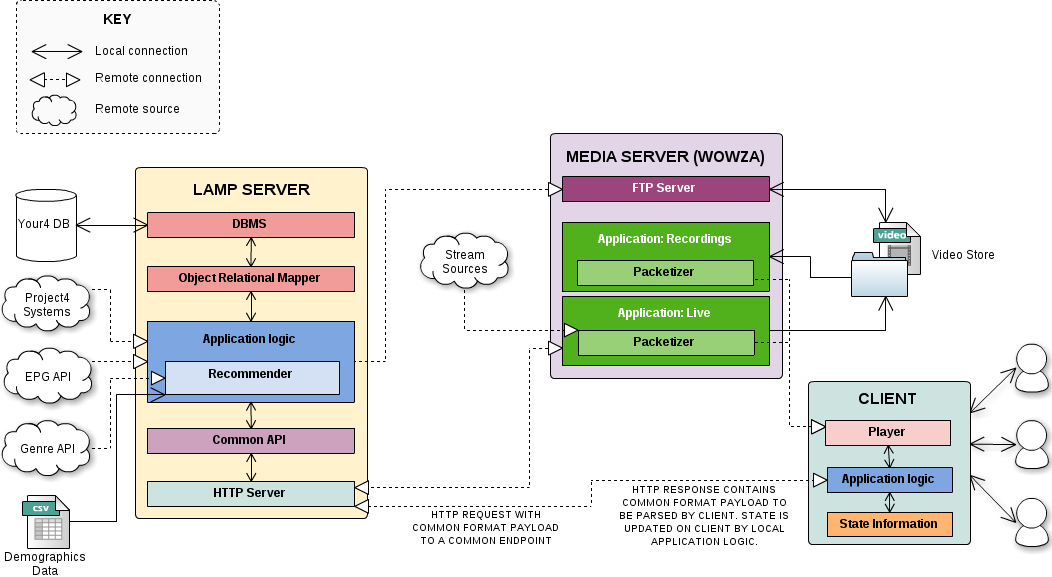
\includegraphics[width=\textwidth]{images/your4-architecture.png}
	\caption{Overview of Your4 architecture}
	\label{fig:your4-architecture}
\end{figure}

Figure~\ref{fig:your4-architecture} shows the overall architecture of the Your4 system. The system is split into three distinct parts:

\begin{description}
	\item[Client] The client (expected to be Mobile Safari for iPad running on top of iOS 5+) is responsible for for interfacing with the LAMP server to retrieve the users' personalised playlist. With this playlist, the player in the client can then request the appropriate media from the media server.
	\item[LAMP server] The LAMP server represents the bulk of the system and is responsible for providing a REST API for the key features of Your4: recommendations, user authentication, electronic programme guide (EPG) data and advert uploading \& manipulation.
	\item[Media server] The media server is responsible for encoding and serving live streams as well as recording programmes and serving recorded programmes.
\end{description}

\subsubsection{Client}

The client receives all HTML content from the LAMP server upon the first visit of your4.tv. From this point onwards, all communication between the client and LAMP server contains only models and collections (e.g. a programme and all of its attributes) on the LAMP servers REST interface in JSON format. The client side application is then responsible for parsing this JSON response and manipulating the user interface using local templates (embedded in the HTML upon the initial page load) as appropriate. Due to the asynchronicity this approach brings, a significant UI speed increase can be observed against traditional methods whereby the web browser acts as a ``thin client'', by simply parsing and rendering HTML responses pre-generated server side.

Using the POST, GET, PUT and DELETE methods in HTTP requests to the REST endpoint maps to the equivalent CRUD (create, read, update and delete) operations on the object concerned. This methodology creates a simple self-documenting API. In a similar exploitation of HTTP philosophies, HTTP status codes are used to identify the status of a request. For example, 200 indicates success and 400 indicates the request was invalid (failed server side validation). The client can then perform the appropriate callback function to manipulate the interface.

\paragraph{Authentication}

The concept of a ``user'' is key to the system since crucial demographics data and matrices defining recommender state are stored against each user. The client authenticates a user by either local login or using the Facebook login API\footnote{\footurl{https://developers.facebook.com/docs/concepts/login}}. Upon page load, the client attempts to retrieve ``/api/users/me'' from the server to discover if an active session is available. If so, the player layers will be rendered on screen, otherwise, the user will be routed to the login interface.

The user can then choose to use the local login which will generate a GET request with the email and password as query parameters. If a 200 response is received, the login is considered to be successful. A user can also choose to login via Facebook. After the user accepts the Facebook permissions, a local cookie is set and a GET request is generated to ``/api/users/fb-[facebook\_id]'' where ``[facebook\_id]'' is retrieved from the Facebook API.

\paragraph{Playback}

Upon initialisation of the player, a number of layers are rendered on top of one another:

\begin{description}
	\item[Video layer] The video component to show video. If on an Apple device, this is a HTML5 video tag. Otherwise, a flash video player is instantiated.
	\item[Skip layer] Contains user controls to skip and rate currently playing media.
	\item[Black layer] Used to hide buffering video in order to provide more seamless stream.
	\item[Overlay layer] An iFrame which displays the HTML that the advertiser has specified to be overlayed on their advert.
\end{description}

Once rendering is complete, the client requests a number of resources from the REST API in order to compile and play a playlist:

\begin{enumerate}
	\item A list of channels including the relevant stream URL to the media server.
	\item The current LAMP server timestamp. This is used in recommendation requests.
	\item A request is made for the best recommended live broadcast. This recommendation is based on the currently playing program on each channel. Live broadcasts are given priority over recorded programmes as this is close to the ``personal TV channel'' ideal. The current timestamp and user ID is sent with this request in order for the server to determine what suitable programmes are upcoming. If a 200 response is received, the body will include the channel ID. If a 404 is received, no appropriate live broadcast recommendation is available. The client will then request a recorded programme recommendation. In both cases, the response also includes the programme ID from the EPG and the location of ad breaks.
	\item With the programme ID, a request is made to retrieve the programme data such as name, description and length.
	\item Between each recorded programme a 2 minute ad break is artificially included. Up to 5 minutes is allowed between live broadcasts (depending on previous programme end and the start of the live broadcast). The system is also aware of ad breaks in programmes within the playlist. For each ad break, a request is made containing: the user ID; programme ID; the amount of time in the ad break; if the ad break is between a live or recorded programme and finally, a list of advert ID's which have already been listed in the playlist. Using this data, the LAMP server can select adverts that match the users demographics and the currently playing programme. This step is repeated multiple times, reducing the amount of time left unallocated in the request each time, until all ad breaks are full.
	\item Steps 3 to 5 are repeated until the minimum duration and size of playlist are both satisfied. Upon each repeat, the timestamp sent with the request is set to the end time of the previously recommended programme or advert. This informs the recommender as to the point in time it should check live broadcasts for suitable programmes.
	\item The playlist is rendered on screen.
	\item The video player is instructed to play the first stream URL in the playlist. Each time an item in the playlist ends, a signal is triggered which causes the player to play the next stream. As well as this, another recommendation is requested and added to the playlist.
\end{enumerate}

The client checks the user agent string of the browser to determine what format of media to request from the media server. Apple devices require HTTP Live Streaming (HLS) streams while the flash player alternative requests an RTMP alternative.

\subsubsection{LAMP server}

The LAMP server's primary responsibility is to expose all required functionality on a single REST endpoint, ``/api''. In general, the LAMP server deals with a request by passing it through various stages before finally manipulating the database:

\begin{enumerate}
	\item A HTTP request is retrieved by the web server.
	\item The request is passed to the REST API where the appropriate function is called dependant on the request URI and HTTP method.
	\item The object in the request body is passed into the Object Relational Mapper.
	\item The ORM builds the approproate SQL query and passes it to the DBMS.
	\item The DBMS modifies or retrieves from the data store.
	\item The application logic returns the result as a HTTP response containing a JSON body.
\end{enumerate}

\paragraph{Authentication}

Upon registration, name, email, gender, date of birth, occupation, postcode and password are required. For Facebook logins, a facebook ID is required in place of the password. Passwords are stored with a Blowfish-based hash type with a per-user 22 character salt and a 1024 iteration cost parameter which prevents rainbow table exploitation in a human lifetime \citep{hashing}. The postcode is converted to latitude \& longitude coordinates based on ordnance survey data. Upon successful authentication, a session cookie is created.

A recommender function is also called which retrieves the user's initial vector. This is based upon the required demographics data provided at registration. This vector is then stored agaist the user in the database.

\paragraph{Programme recommendations}

Daily, EPG data is imported from the Atlas API\footnote{\footurl{http://atlas.metabroadcast.com}} into the Your4 database. This contains unique programme ID's, descriptions, start and end times, episode numbers, and other programme data.

Upon first initialisation of the recommender, a CSV file containing training data from the GroupLens research group\footnote{\footurl{http://www.grouplens.org/node/73}} is processed. This gives the recommender an initial estimate as to what type of users prefer what genres. Upon execution of the aforementioned EPG cron job, each programme is passed to a recommender function to retrieve the initial programme vector to store against it. This function calls the genre API, TVDB\footnote{\footurl{http://thetvdb.com}}, to identify this vector. The vector is a 1-dimensional matrix whereby each position represents a predefined genre. A ``1'' indicates the programme belongs to a genre.

Upon receiving a live recommendation request, the recommender selects programmes starting within the next 5 minutes of the timestamp contained in the request (see step 3 in aforementioned playback steps). The recommender then filters out programmes the requesting user has already viewed in the past, and selects the best one according the recommender output. If no suitable live recommendation can be made, a 404 will be returned and the client will request a recorded programme. The recommender then executes a similar process to the live request, but filters programmes by those which have been recorded by the media server.

When a user rates a programme on the client, a request is received by the recommender. This rating is a 5-star system which maps to -1, -0.5, 0, 0.5 and 1 respectively. Upon this request, the recommender tunes the users vector accordingly. The act of rating also adds the programme to the list of already viewed programmes for a user.

\paragraph{Adverts}

Inqb8r's Project4 hardware systems receive XML data pertaining to the times ad breaks are positioned during programmes as described in \ref{subsubsec:Project4Tech}. The information (known as a MOS record) is also stored in the Project4 MySQL database. Excluding network delays, we are able to discover the existence of ad breaks up to 1 minute and 8 seconds before they are shown. This information is imported regularly into the Your4 database and made available via the REST interface. With this data, the client is able to know at which points in time it should request an advert to replace the adverts provided in stream by the broadcaster.

Upon uploading of an advert to Your4 by an advertiser, an FTP session is instantiated by the LAMP server to the media server. The advert is then uploaded to the media server where it is stored alongside other adverts and recorded programmes in the video store. An interactive overlay can also be specified, which will be used in the body of the iFrame element of the overlay layer during playback. Campaign information such as target locations, programmes, gender, age and other specifics can also be specified for storage against the advert in the Your4 database. The advertiser can also specify the times of day (on a per-day basis) and the programmes that they wish their advert to be shown in.

When the client requests an advert, the amount of time the advert has to fill and the ID's of adverts that have already been scheduled in the ad break are included in the request. The LAMP server then performs a search on the database for adverts that match these characteristics (duration less or equal than the remaining ad break time left and the advert has not been shown already in this ad break) and the targeting criterion set by the advertiser. Any adverts the user has shown a dislike for in the past will also be filtered out.

Views, clicks and skips are recorded by the client and feedback is sent to the REST interface. The advertiser can then view these statistics.

\subsubsection{Media server}

Video streams are delivered to the client via a Wowza media server\footnote{\footurl{http://www.wowza.com/}}, hosted on a Windows Server 2008 based machine. This machine is provided by Inqb8r, who have extensive experience with Wowza based systems.

The Wowza server is configured to act as a repeater, re-broadcasting the streams provided by Inqb8r. This server is based on two distinct applications. The first application is responsible for retrieving the source live streams and relaying these to the client. The second is responsible for streaming recorded programmes and adverts from the video store to the client (the standard wowza extension ``vod'' allows any file of a valid format in a given directory to be streamed). Both applications use a ``packetizer'' which is responsible for encoding the raw input streams to the output requested (HLS for Apple based devices). The packetizer is chosen based on this request, for example, the ``cupertino'' packetizer is used to encode Apple HLS streams.

The live application is also responsible for recording programmes. The LAMP server's EPG REST interface is continuously polled for any shows due to start in the next minute to retrieve the start and end times of programmes. Using this data, the application records each programme on each channel and stores the resulting media in the video store. This media is stored with a filename which matches that of the unique ID in the EPG. This allows the client to implicitly build the video URL to request when a recorded programme recommendation is made. When a recording starts, the application updates the ``recordState'' flag of the programme via the REST interface. This flag is updated again when recording is completed. Using the state of this flag, the recommender is able to filter out programmes which have not yet been recorded during recorded programme recommendation. The recordings application can then stream these media files to the client when requested.

Recording is processed by the Wowza ``LiveStreamRecord'' module. This module imposes a strict limit of only one simultaneous recording per stream. When a new programme starts any current recording on the channel is stopped, ensuring this enforced mutual exclusion. The end result is a set of video files for each programme stored in the video store.

As every programme is recorded, scalability in terms of storage is an issue. For this reason, recorded video's are removed after a configurable amount of time. First, the recording is removed from further recommendations by setting the ``recordState'' flag of the programme to ``deleted'' via the REST interface. After an amount of time equal to the length of the video has passed, the video file itself is removed. This allows any existing viewers of the recording to complete their viewing of the programme.

\subsection{Database structure}

\begin{figure}[H]
	\centering
	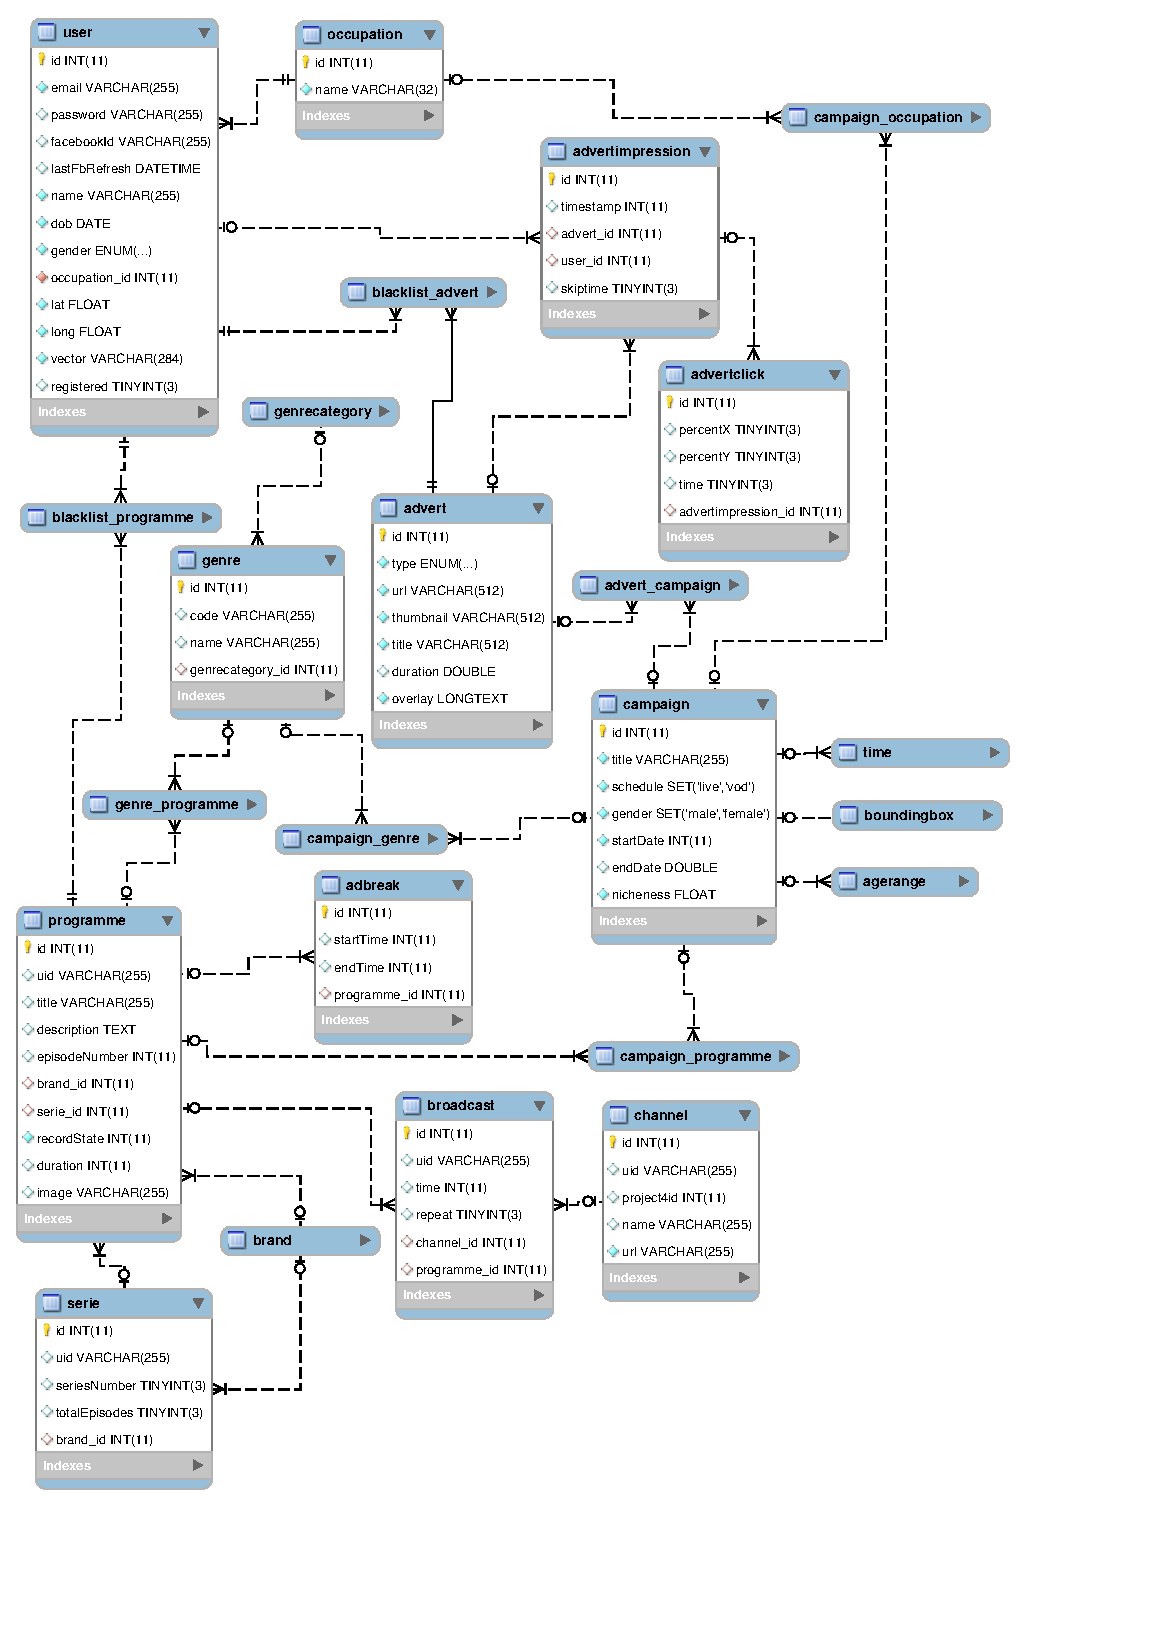
\includegraphics[trim = 0 3.7cm 3.5cm 0, clip, width=\textwidth]{images/your4-db.pdf}
	\caption{Overview of Your4 database layout}
	\label{fig:your4-db}
\end{figure}

Figure~\ref{fig:your4-db} shows the Your4 database class diagram. The Object Relational Mapper (ORM) in use enforces a strict naming policy in which all table and attributes are in lower case and are not pluralised. The underscore character represents a relation, e.g. ``programme\_id'' represents a foreign key to the ``id'' attribute in the programme table.

\subsection{Programming techniques and languages}

The implementation consists of a number of subsystems using different programming languages. The client is built on JavaScript, HTML and CSS; the LAMP server on PHP for the REST interface and Python for the recommender; and finally, the media server is based on a Java implementation. In order to achieve a concise and maintainable solution, a combination of design strategies and good use of libraries was employed.

\subsubsection{Design strategies and Patterns}

Where possible, it is good practice to use popular design strategies and patterns as templates to solve common problems in application development. A number of such strategies were used during the implementation stage, the most prevalent of which are documented here:

\begin{description}
	\item[MV*] By seperating models and views using the client-side Backbone.js library, the client is easily able to retrieve objects (models) from the REST interface and attribute them to a view. The view can then use the attributes of the model to render the appropriate HTML in the DOM. This view can also handle user manipulation and edit the models attributes. Models can be swapped in and out of a view easily, and the result re-rendered on screen.
	\item[Front controller] By using a client-side URL router, navigation is controlled by a single object. This allows for easy tracking and manipulation of the current application navigation state. This router then calls the appropriate function relevant to the currently visited route.
	\item[Observer pattern] By allowing objects to subscribe to and trigger events, signals can be passed to an object or set of objects without tight coupling. For example, a signal is sent to the player view when an item in the playlist is due to start. As well as the player view, the views representing the playlist are also subscribed to the event, so they can shift the ticker (representing time elapsed on the playlist) to the start of the next programme.
	\item[Facade pattern] The LAMP REST interface maps HTTP methods to the equivalent CRUD operations on the object contained within the request body. By providing this self-documenting ``facade'', the inner complexities and domain-specific operations are hidden from the external API.
\end{description}

\subsubsection{Libraries and frameworks}

A number of libraries and technologies were used during the implementation stage:

\begin{description}
	\item[Client] \hfill
		\begin{description}
			\item[JQuery] JQuery allows simple DOM manipulation and event handling.
			\item[Underscore] A JavaScript library which introduces functional programming aspects with significant performance benefits.
			\item[Backbone] A Model-View-Controller type framework to interface with REST services.
			\item[Flowplayer] The Flash player used for non-Apple devices.
			\item[Bootstrap] A CSS framework defining sensible cross-browser styling.
			\item[D3] Visualisation library which provides graphing capabilities (SVG manipulation).
			\item[Leaflet] Mapping for mobile touch screen devices.
			\item[Facebook] Used for Facebook login functionality.
		\end{description}
	\item[LAMP Server] \hfill
		\begin{description}
			\item[MySQL] Relational DBMS for primary storage.
			\item[Slim] PHP framework used to implement REST interface and application logic.
			\item[RedBean] PHP Object Relational Mapper for easy database manipulation.
			\item[Facebook] Used for validating facebook logins.
			\item[TVDB] Used by the recommender to retrieve programme genres.
			\item[NumPy] Used by the recommender for manipulation of matrices.
		\end{description}
	\item[Media Server] \hfill
		\begin{description}
			\item[Wowza] Java media server.
			\item[LiveStreamRecord] Wowza module to allow recording of live streams to files.
			\item[Gson] Java library used to convert objects to and from JSON for the REST interface.
		\end{description}
\end{description}


\subsubsection{Code statistics}
Lines of code in JS, PHP, Java, Python, HTML, CSS etc
\begin{center}
	\begin{tabular}{l r r r}
		\toprule
		\textbf{Language} & \textbf{Files} & \textbf{Comments} & \textbf{Code} \\
		\midrule
		JavaScript & 11 & 55 & 2686 \\ 
		PHP & 26 & 28 & 1515 \\ 
		Python & 17 & 282 & 1239 \\ 
		Java & 20 & 322 & 1056 \\ 
		CSS & 5 & 18 & 603 \\ 
		HTML & 2 & 8 & 462 \\ 
		XML & 4 & 100 & 151 \\ 
		\midrule
		sum & 85 & 681 & 7714 \\ 
		\bottomrule
	\end{tabular}
\end{center}


\subsection{System walkthrough}
\begin{figure}[th]
	\centering
	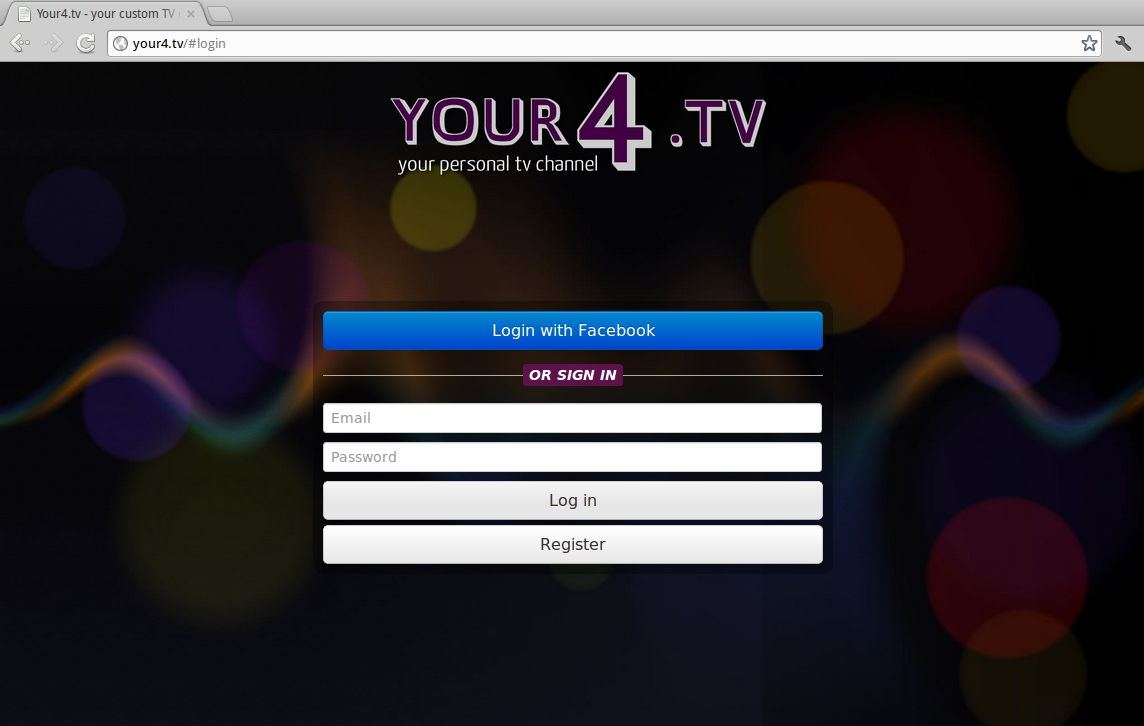
\includegraphics[width=\textwidth]{images/screenshots/your4-login.png}
	\caption{Log in}
	\label{fig:your4-login}
\end{figure}
\begin{figure}[th]
	\centering
	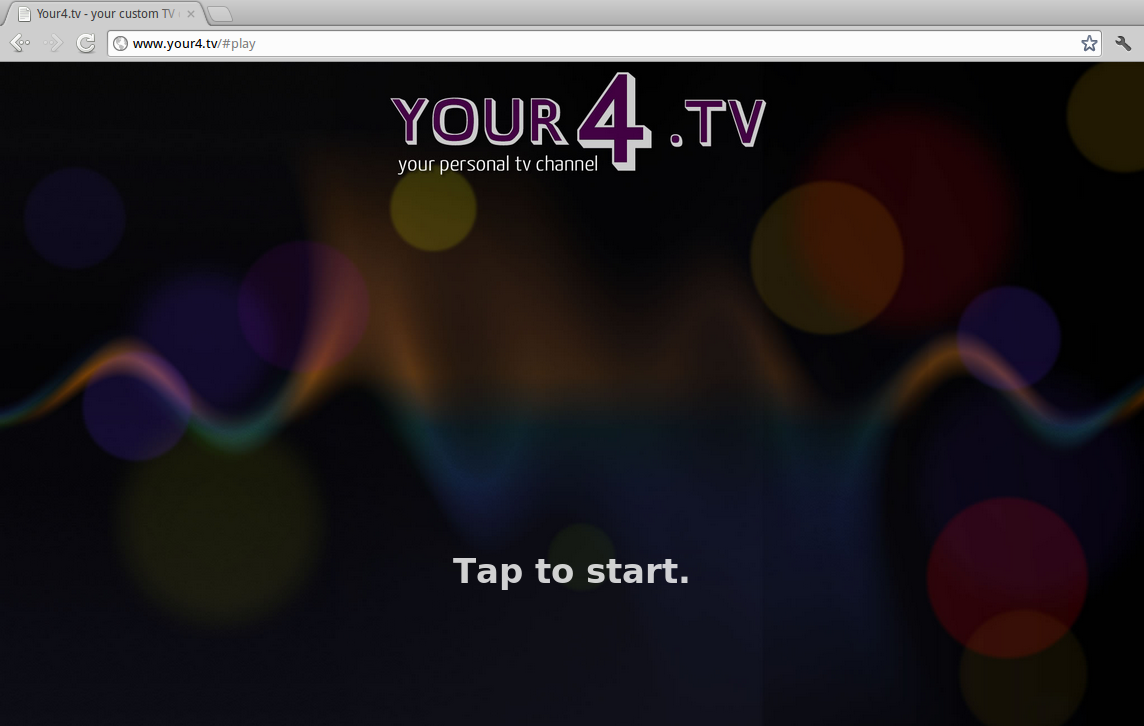
\includegraphics[width=\textwidth]{images/screenshots/your4-tap-to-start.png}
	\caption{Log in}
	\label{fig:your4-tap-to-start}
\end{figure}
\begin{figure}[th]
	\centering
	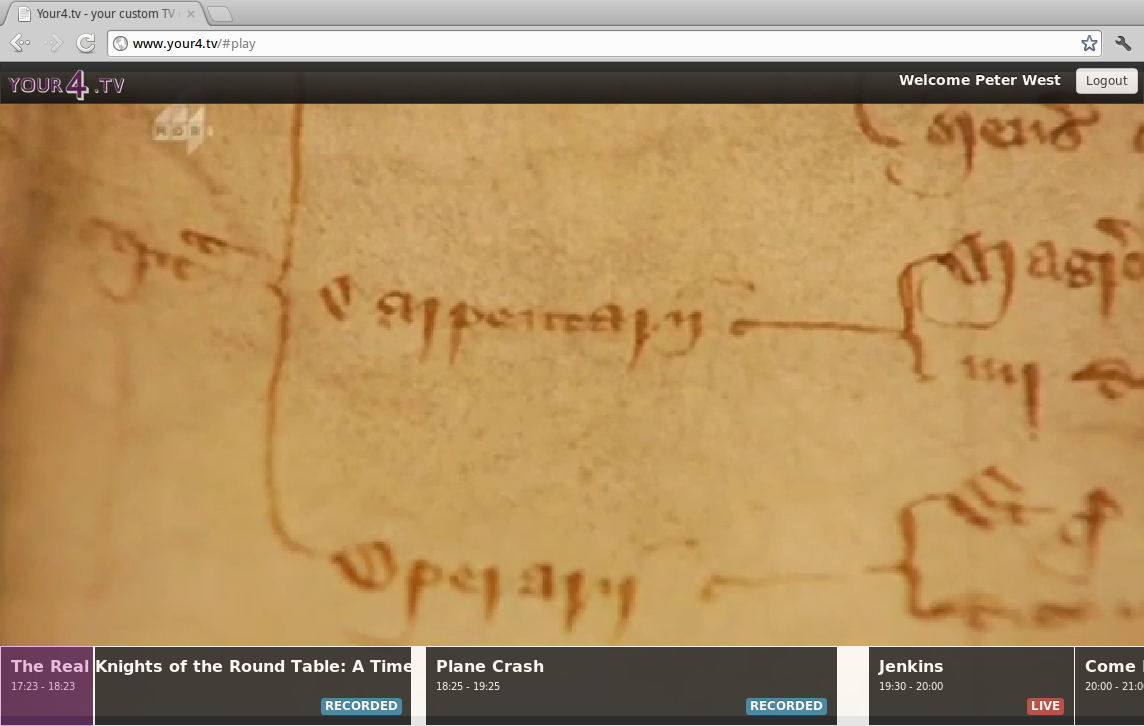
\includegraphics[width=\textwidth]{images/screenshots/your4-play.png}
	\caption{Log in}
	\label{fig:your4-play}
\end{figure}

\begin{figure}[th]
	\centering
	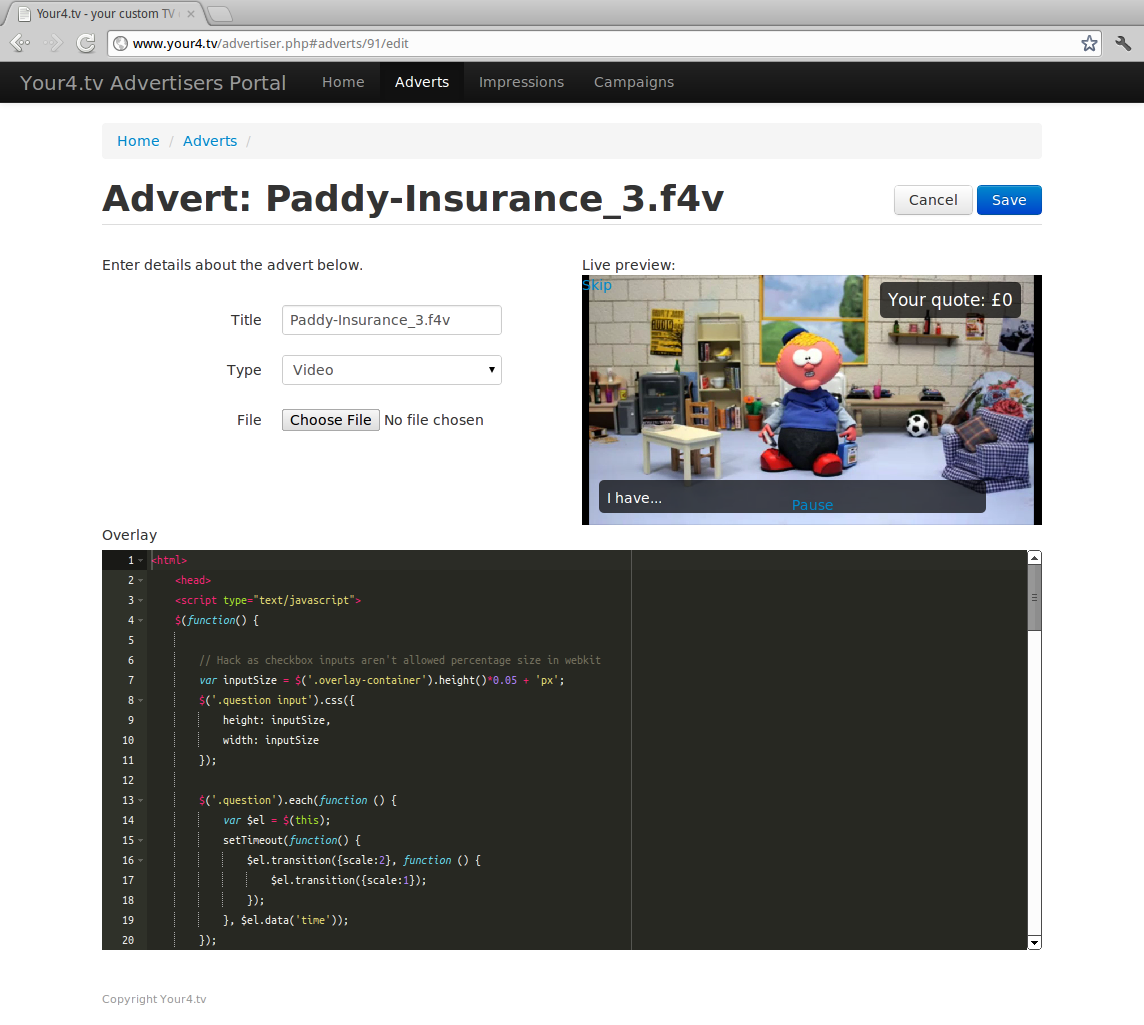
\includegraphics[width=\textwidth]{images/screenshots/advertiser-advert-edit.png}
	\caption{Log in}
	\label{fig:advertiser-advert-edit}
\end{figure}
\begin{figure}[th]
	\centering
	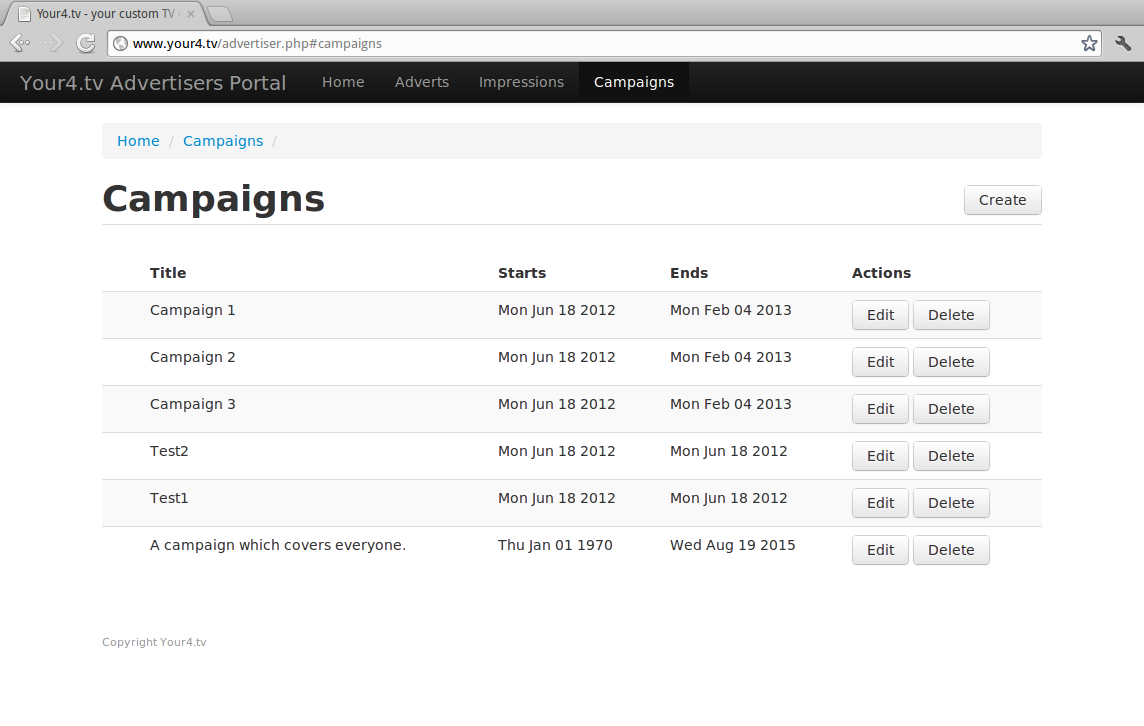
\includegraphics[width=\textwidth]{images/screenshots/advertiser-campaigns.png}
	\caption{Log in}
	\label{fig:advertiser-campaigns}
\end{figure}
\begin{figure}[th]
	\centering
	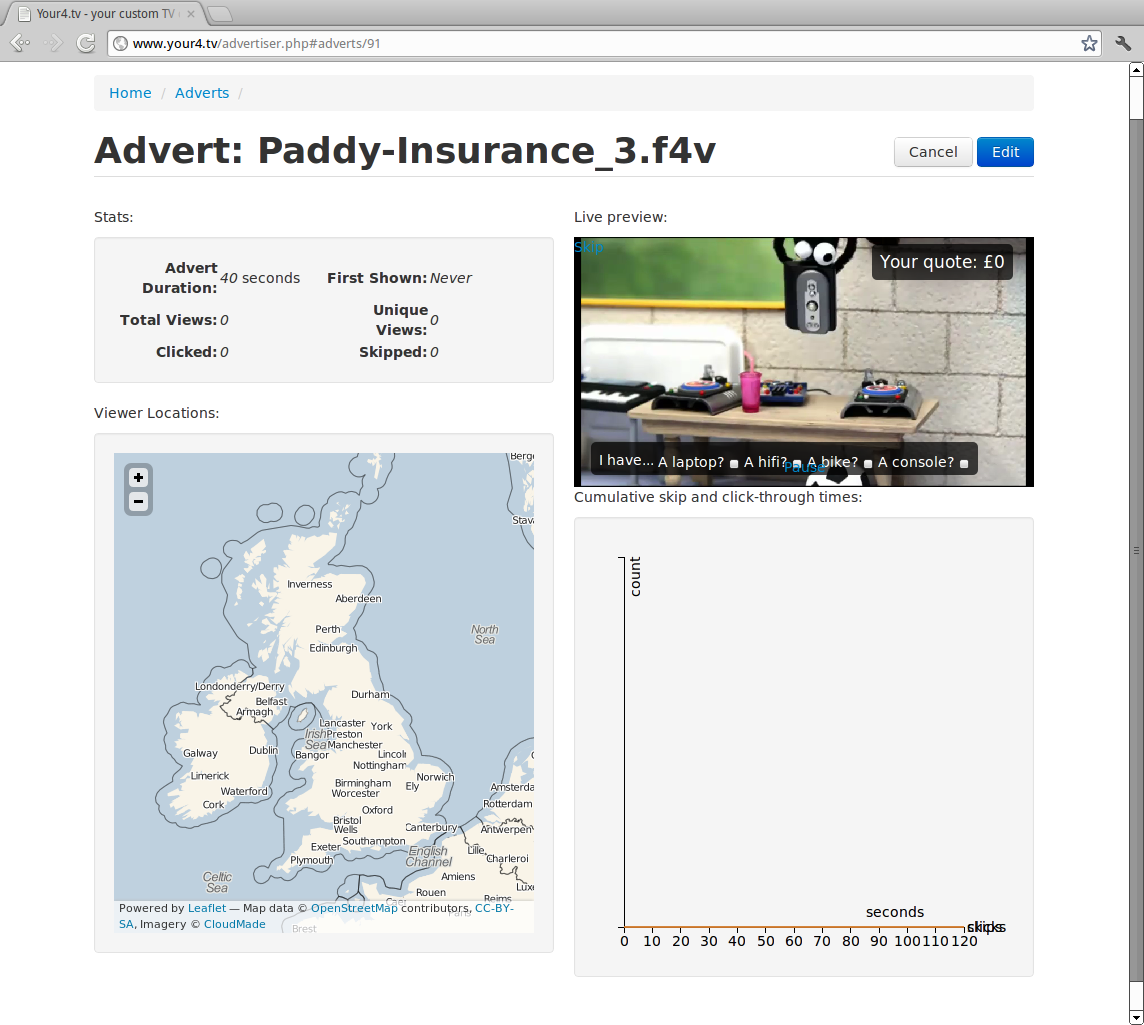
\includegraphics[width=\textwidth]{images/screenshots/advertiser-advert.png}
	\caption{Log in}
	\label{fig:advertiser-advert}
\end{figure}
\begin{figure}[th]
	\centering
	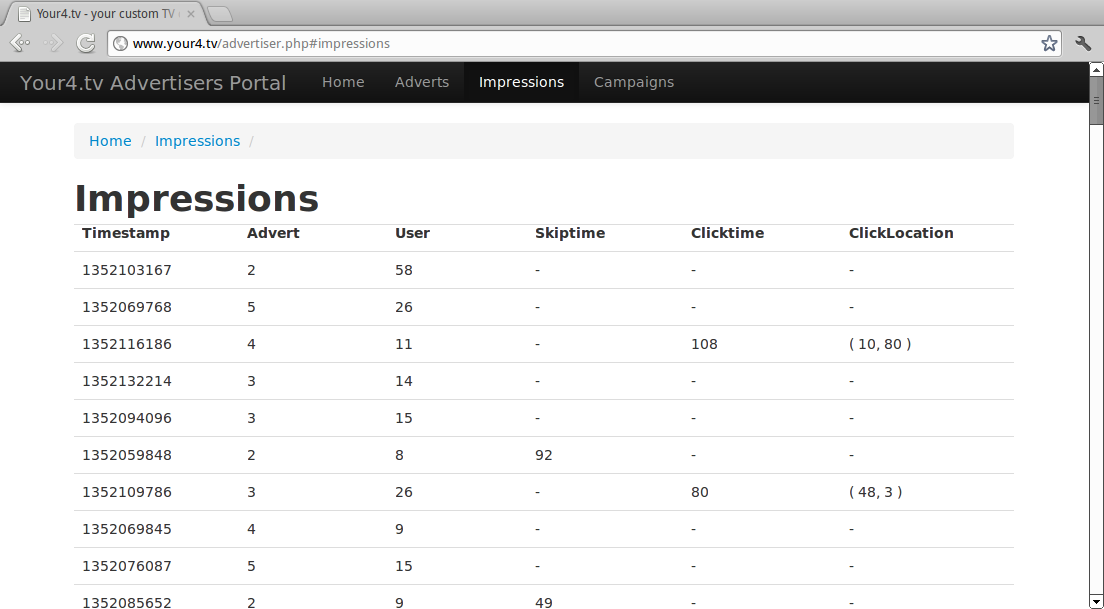
\includegraphics[width=\textwidth]{images/screenshots/advertiser-impressions.png}
	\caption{Log in}
	\label{fig:advertiser-impressions}
\end{figure}
\begin{figure}[th]
	\centering
	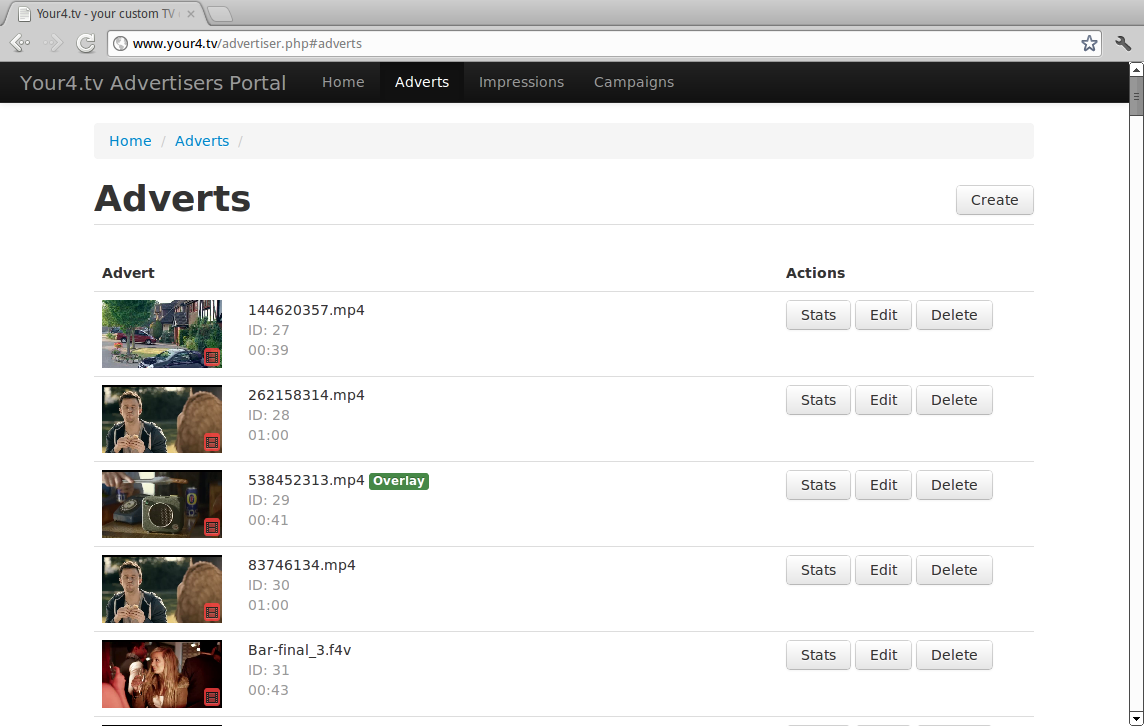
\includegraphics[width=\textwidth]{images/screenshots/advertiser-adverts.png}
	\caption{Log in}
	\label{fig:advertiser-adverts}
\end{figure}
\begin{figure}[th]
	\centering
	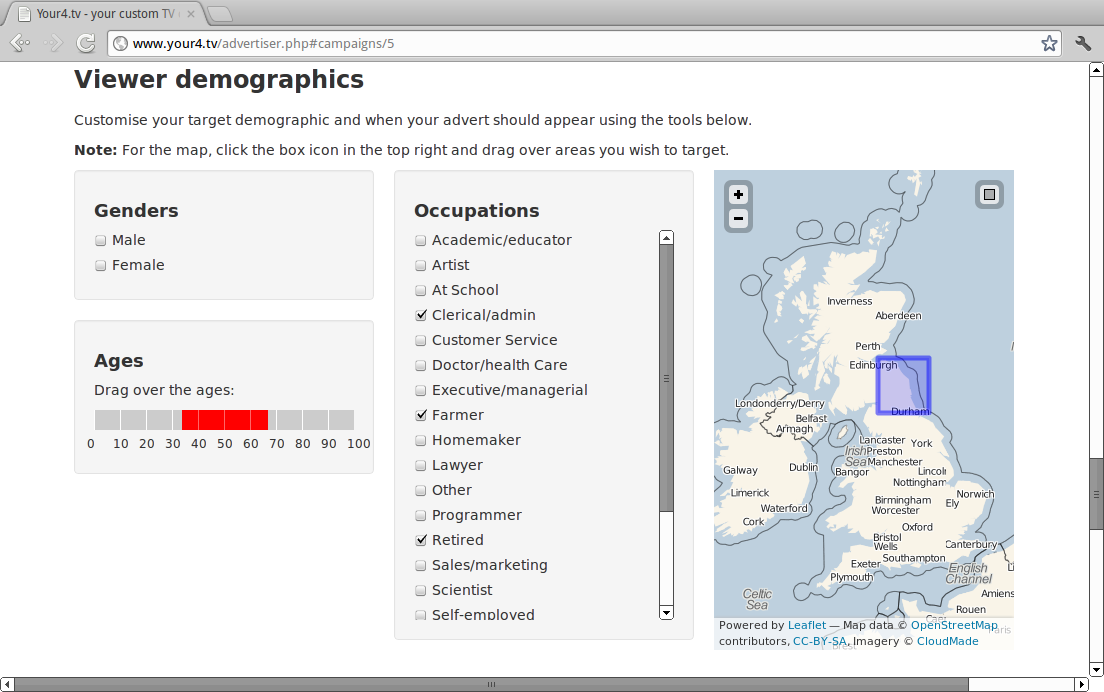
\includegraphics[width=\textwidth]{images/screenshots/advertiser-campaign-demographics.png}
	\caption{Log in}
	\label{fig:advertiser-campaign-demographics}
\end{figure}
\begin{figure}[th]
	\centering
	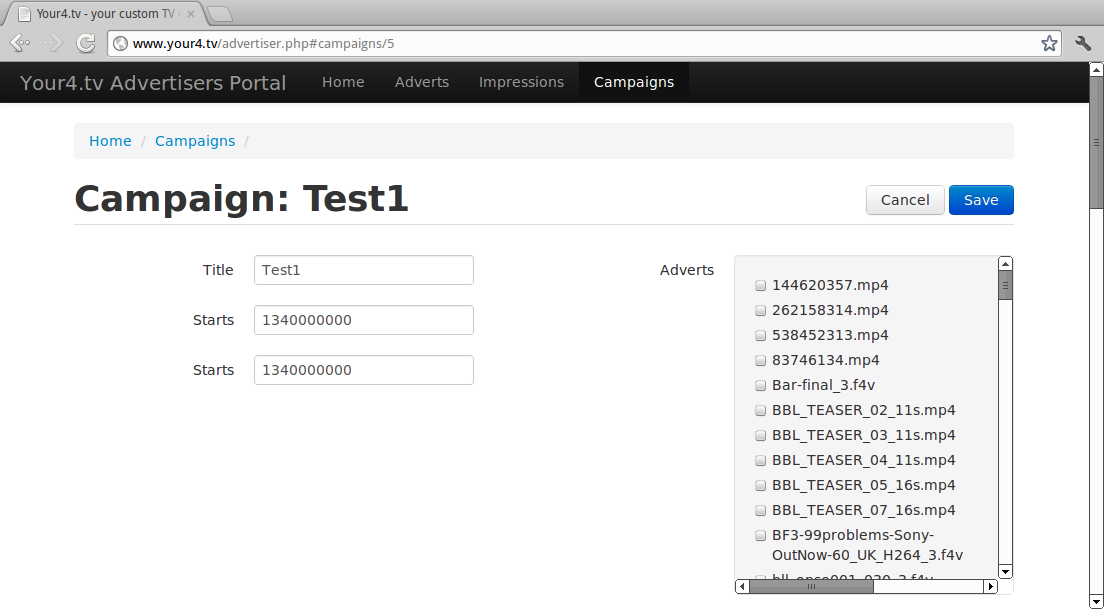
\includegraphics[width=\textwidth]{images/screenshots/advertiser-campaign.png}
	\caption{Log in}
	\label{fig:advertiser-campaign}
\end{figure}
\begin{figure}[th]
	\centering
	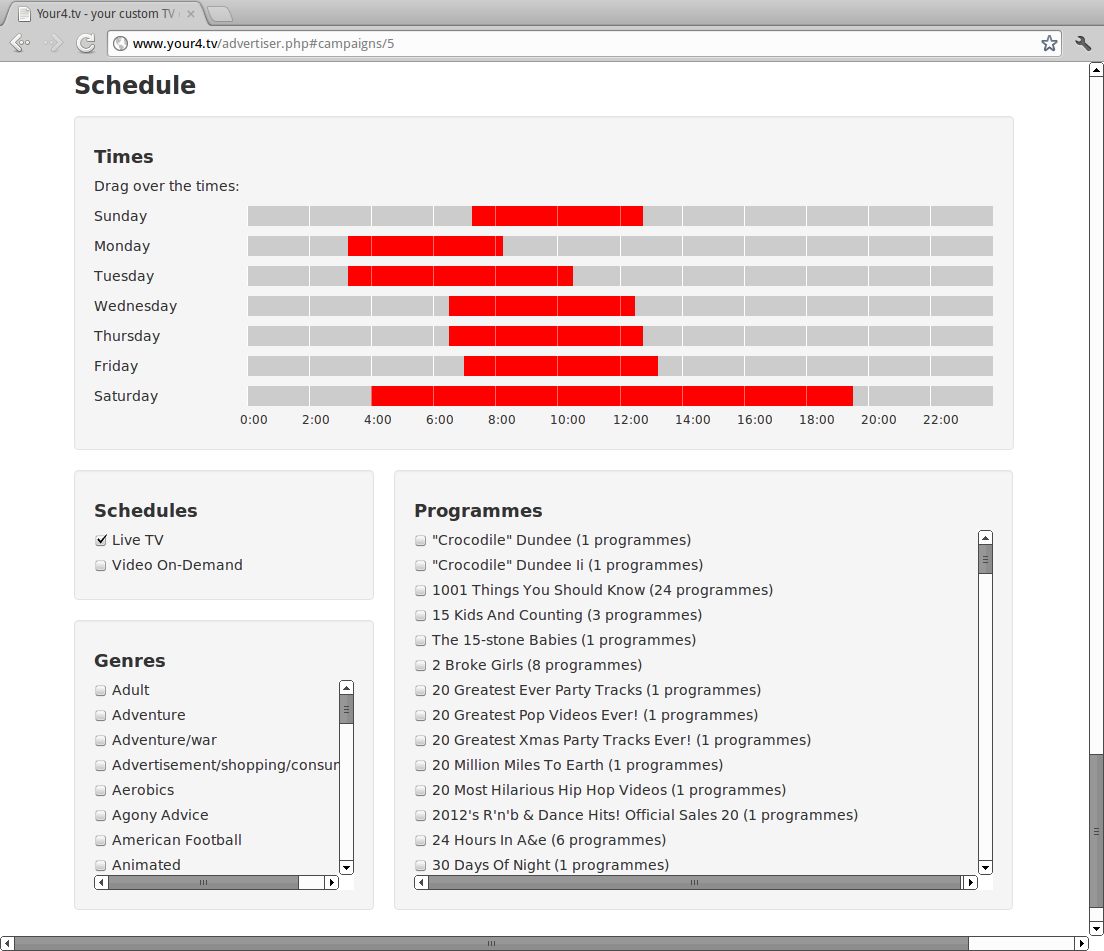
\includegraphics[width=\textwidth]{images/screenshots/advertiser-campaign-schedule.png}
	\caption{Log in}
	\label{fig:advertiser-campaign-schedule}
\end{figure}
